\documentclass[twocolumn,a4paper]{ctexart}

\usepackage{amsmath,amssymb,amsfonts}
\usepackage{graphicx}
\usepackage{booktabs}
\usepackage{url}
\usepackage[margin=1.8cm]{geometry}
\usepackage{abstract}
\graphicspath{{figures/}}

\title{\bfseries 面向智能体的大模型自进化强化学习系统}
\author{孙豪\\[2pt] \normalsize 中国人民大学\ 智慧治理学院}
\date{}

\begin{document}

\twocolumn[
\maketitle
\begin{onecolabstract}
\noindent\textbf{摘要}\quad 大语言模型驱动的智能体在代码沙箱、文件系统等真实环境中通过多步工具调用完成任务，强化学习是让其持续变强的主流手段。然而，交互式智能体的强化学习面临一个根本性瓶颈：训练数据与可信奖励均难以靠人工规模化获得——真实用户数据积累慢、覆盖窄，而奖励若仅依赖智能体自述，模型会迅速习得谎报完成这一奖励作弊行为。本文提出一套面向智能体的\emph{自进化}强化学习系统，使智能体在无人工标注条件下自主产生训练数据、自主获得可信奖励、自主生成下一轮训练任务。系统包含四个核心机制：（1）由三智能体协作与沙箱状态真继承驱动的跨步自进化任务生成；（2）将打分锚定在确定性环境状态差分而非自述的差分驱动奖励；（3）每步只保留梯度最优轨迹子集的超采样-淘汰-选组；（4）失败案例驱动的评估器与基建自演化。系统在 Qwen3.5-9B 上端到端验证，完整链路仅由少量种子驱动、除初始种子外不依赖任何外部数据；离线评测进一步确认训练带来的是相对未训练基座的真实能力提升，而非仅训练指标好看。

\vspace{4pt}
\noindent\textbf{关键词}\quad 大语言模型智能体；强化学习；自进化；奖励作弊；GRPO
\vspace{10pt}
\end{onecolabstract}
]

\section{引言}

随着大语言模型能力与应用场景不断扩展，依赖人工构造任务和固定数据集的传统训练范式面临扩展瓶颈：固定数据难以覆盖不断增长的任务空间，而交互式智能体的强化学习持续消耗新的交互轨迹，使数据获取成为限制训练规模与持续迭代的关键因素。\emph{自进化}正是对此的回应——使模型在极少人工干预下，通过“生成—执行—评估—反馈—更新”的循环不断产生新经验并优化自身\cite{self_evolution_survey,self_improve}。

自进化在两个层面展开。在\textbf{模型层面}，模型自行生成数据、自我评分、筛选后微调自身，衍生出自我博弈、自我奖励、RLAIF、拒绝采样、进化搜索等范式\cite{self_play,self_rewarding,rlaif,absolute_zero}；在\textbf{智能体层面}，智能体在环境中积累经验，持续改进记忆、技能库、工具使用、提示词与规划策略，乃至底层模型参数。本文系统同时贯通二者：既让模型自主生成数据、以环境真实状态为准自我评分、经强化学习更新参数，又让智能体在沙箱中积累经验、以失败案例驱动评估提示词与工具/基建的持续演化。

然而，当任务生成、奖励评估与策略更新均由系统自动完成时，训练闭环也面临新的风险：评估偏差或低质数据会随后续轮次被放大\cite{reward_hacking_def,reward_overoptimization}——智能体可能通过迎合评估器偏好获得高分而实际未完成任务。因此，自进化系统不仅需要持续产生数据，还需建立与环境执行结果相结合的奖励评估，并对候选经验进行质量控制。本文的主要贡献为：

\begin{itemize}
\item \textbf{跨步自进化任务生成}：让每个新任务生长在上一轮真实产物之上，除初始种子外自主产生所有后续任务。
\item \textbf{多智能体自主数据生成}：使采样、取证、追问全部自主化。
\item \textbf{差分驱动奖励}：将打分锚定在确定性环境状态差分，从取证机制上抑制奖励作弊。
\item \textbf{失败案例驱动的评估器与基建自演化}：将自进化从任务与策略扩展到评估器与基建四维。
\item 在 Qwen3.5-9B 上的\textbf{端到端验证}：闭环可自我维持并带来真实能力提升。
\end{itemize}

\section{系统概述}

系统由三个协同智能体（执行者、观察者、提问者）、代码沙箱、外部冻结裁判~\cite{llm_judge}与 GRPO 训练器~\cite{grpo}组成。执行者以 ReAct 方式推理与行动~\cite{react}、并以可执行代码为动作空间~\cite{codeact}。全部自定义采样与选组逻辑通过强化学习框架的官方注入点接入，与框架主体解耦。总体架构如图~\ref{fig:arch} 所示。

\begin{figure}[t]
\centering
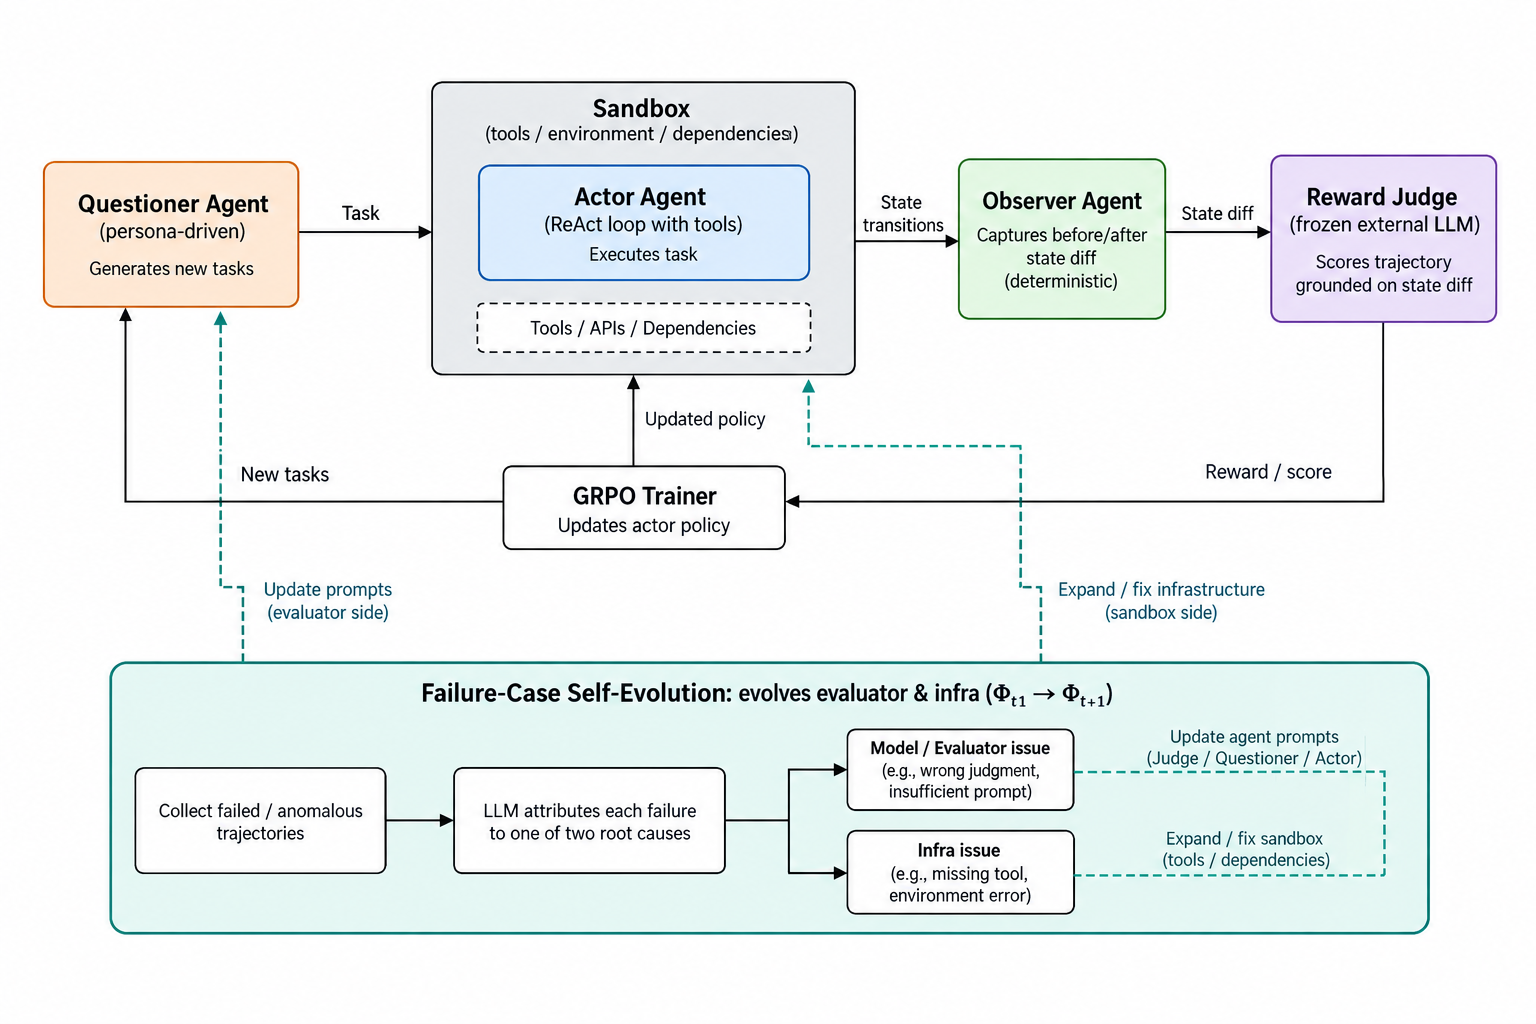
\includegraphics[width=\columnwidth]{arch.png}
\caption{系统总体架构：三协同智能体、代码沙箱、冻结裁判与 GRPO 训练器，经框架注入点接入。}
\label{fig:arch}
\end{figure}

将自进化过程建模为转移算子 $\mathcal{T}$ 在系统状态 $\sigma_t=(\theta_t, s_t, Q_t, \Phi_t)$（策略参数、沙箱状态、任务集、评估器/基建状态）上的反复作用。一个训练步内主循环分三阶段：
\begin{align}
Q_t &\xrightarrow{\ \pi_{\theta_t}\ } \tau_t \xrightarrow{\ \text{Observer}\ } d_t, \\
d_t &\xrightarrow{\ \text{Judge}(\cdot;\Phi_t)\ } R_t \xrightarrow{\ \text{GRPO}\ } \theta_{t+1}, \\
(\tau_t, d_t) &\xrightarrow{\ \text{Questioner}\ } Q_{t+1}.
\end{align}
主循环之外，评估器/基建状态 $\Phi_t$ 由失败案例集 $\mathcal{B}_{t'}$ 驱动、按低频演化。传统强化学习是其退化情形（$Q_t\!\equiv\!Q_0$、$s_t\!\equiv\!s_0$、$\Phi_t\!\equiv\!\Phi_0$，仅 $\theta_t$ 演化）；本文系统同时演化四个维度。

\section{方法}

\subsection{跨步自进化任务生成}

本机制使系统除初始种子外自主产生所有后续任务，核心是\emph{让下一轮任务生长在上一轮真实执行结果之上}。每步结束后，对每个存活组取奖励最高的轨迹及其沙箱状态；观察者视随机策略概括该轨迹的“意图—产物—缺口”；沙箱文件系统状态被真继承到新沙箱（真状态继承而非文本描述）；人设驱动的提问者据此生成下一轮种子。闭环如图~\ref{fig:selfevolve} 所示。

\begin{figure}[t]
\centering
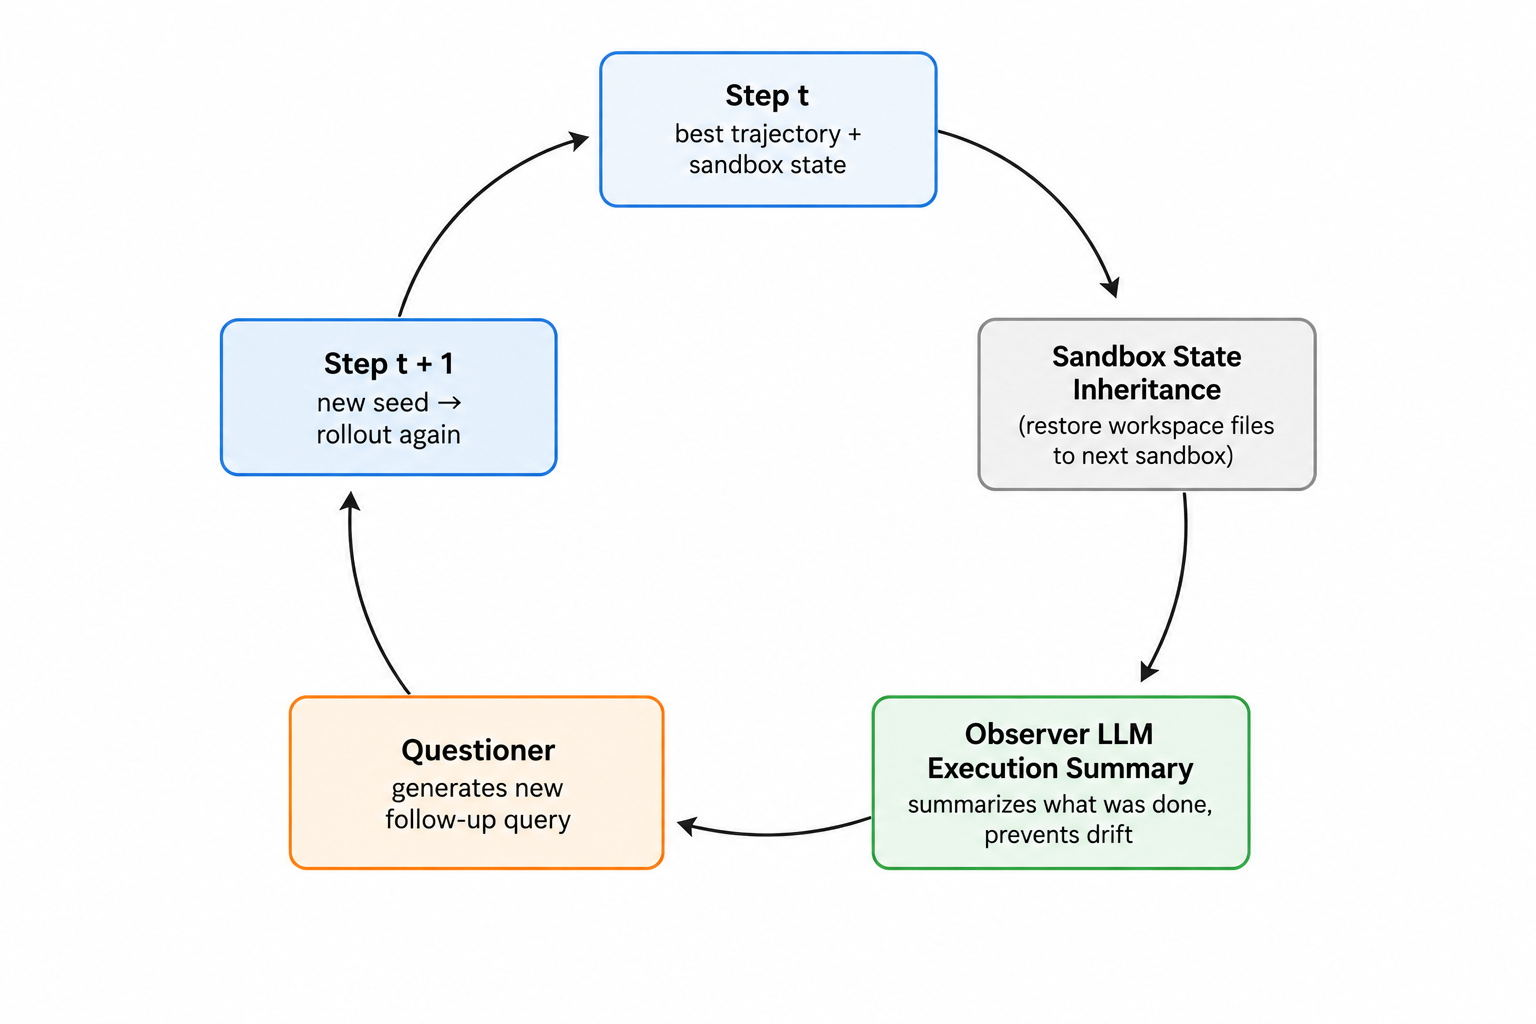
\includegraphics[width=\columnwidth]{selfevolve.png}
\caption{跨步自进化：最优轨迹的沙箱状态被继承，提问者基于执行概括生成下一轮任务。}
\label{fig:selfevolve}
\end{figure}

执行概括设为\emph{随机启用}，由此产生两种互补任务模式：\emph{延续模式}（启用概括）把已有工作延伸成长程任务链，\emph{新任务模式}（不启用）仅面对继承环境提出全新任务。以概括替代原始轨迹是有意的——将旧策略轨迹原文拼入新策略上下文会引入离策略偏差与分布偏移，而概括只保留剥离了旧策略生成痕迹的任务层信息。

\subsection{多智能体自主数据生成}

三个职责分离的智能体把一次采样变成完整的“提问—执行—取证”交互（图~\ref{fig:multiagent}）。\textbf{执行者}（被训练策略）在沙箱中以 ReAct 求解任务；\textbf{观察者}在执行前后各拍只读快照、作差得到确定性状态差分，只依据环境证据而不采信自述；\textbf{提问者}扮演人设驱动的模拟用户生成下一轮种子。求解与追问是开放性生成，取证要求客观不可操纵——这种“能力与确定性分离”正是差分驱动奖励可信的基础。训练数据由系统内各单元的相互博弈动态产生，是一种以真实沙箱为环境、以环境状态而非纯文本为裁决依据的自我博弈。以角色分工的智能体生成交互数据的思路与 CAMEL~\cite{camel} 及多角色自进化（如 R-Zero~\cite{r_zero}）一脉相承。

\begin{figure}[t]
\centering
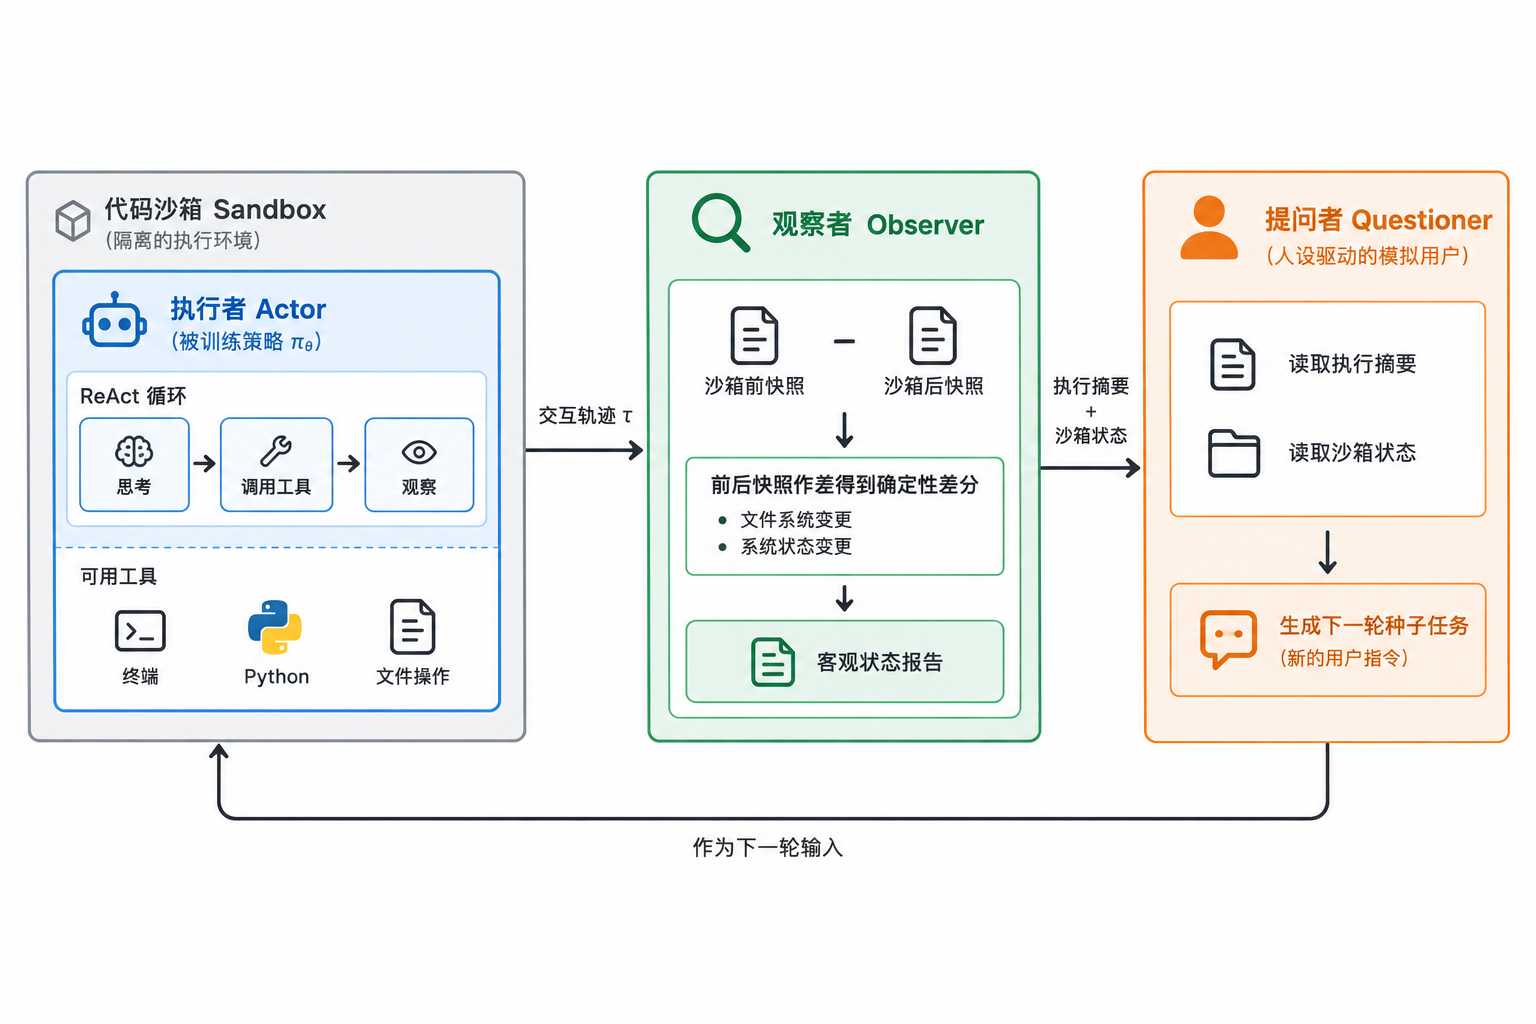
\includegraphics[width=\columnwidth]{multiagent.png}
\caption{多智能体协作数据生成：执行者、观察者、提问者串接在同一沙箱会话上。}
\label{fig:multiagent}
\end{figure}

\subsection{超采样-淘汰-选组}

为提升每步信号质量，将推理与训练解耦。每步超采样 $S$ 个种子 $\times\,n$ 条轨迹；淘汰同时满足“最大奖励处于后 20\%”且“低于阈值”的组（至少保留 80\%）；对存活的 $R$ 组按组内优势绝对值均值排序，取前 $N$ 组做 GRPO。这一“动态采样、过滤无效组”的思路与 DAPO~\cite{dapo} 一脉相承。依据在于：GRPO 梯度由组内优势驱动，零方差（全对/全错）组不贡献有效更新；在固定预算下选高信号子集可最大化每步策略改进。

\subsection{差分驱动奖励}

将打分的证据基准从“智能体说了什么”换成“环境里真实发生了什么”。冻结裁判依据观察者的确定性状态差分（文件系统与系统状态变更）打分，自述仅作交叉核对。评分采用多维度乘性聚合（完成度、正确性、轨迹质量），任一关键维为零则总分为零；安全维为二元门；空差分直接短路为 0、不调裁判。形式化地，对任何仅改变自述、不改变状态差分的行为 $\delta$（$d(\delta)=d$），有 $\mathbb{E}[R\mid\delta]=\mathbb{E}[R]$：纯话术作弊被完全阻断，任何奖励提升都必须以真实的环境改变为前提。

\subsection{失败案例驱动的评估器与基建自演化}

除任务与策略外，完整的自进化智能体还应演化其\emph{评估器}（打分/提问提示词）与\emph{基建}（工具、沙箱、执行环境）。已有工作表明失败可经语言化反思归因与修复~\cite{reflexion}、缺失能力可沉淀为可复用技能库~\cite{voyager}。在此基础上，系统周期性收集失败案例（执行失败、奖励异常、自述与差分矛盾）；每 10 步或攒够 20 例，由大模型将根因归于\emph{模型侧}（规划、工具使用、方案选择）或\emph{基建侧}（缺依赖、缺工具、超时过短、harness 缺陷），据此分别对提示词做增量修订、或将缺失能力沉淀为可复用技能。

\subsection{自进化稳定性控制}

系统无人值守运行，在现有计算路径上监控五项坍缩指标：奖励标准差、优势标准差、策略 KL、训练损失（NaN/Inf）、存活组数。任一触发即终止——各指标对应不同失稳模式，任一单独触发都意味继续运行只会浪费算力。

\section{实验}

\subsection{设置}

基座为 Qwen3.5-9B，采用标准 GRPO，推理与训练异步解耦。正式训练用 2 节点 $\times$ 8 卡 H800，每步 $N{=}64$ 组，运行 50 步（为与传统 RL 对比而手动结束；系统本身除稳定性判据外不限制步数）。下文结果均来自\emph{同一次}端到端实验，只是从不同维度观察。

\subsection{闭环自我维持与奖励}

超采样量 $S$ 单调收缩并稳定在 $N$ 附近而不塌缩至零，各步跨步种子均成功生成——在无外部数据补给下闭环可自我维持。图~\ref{fig:reward} 在完全相同的 GRPO 管线下对比自产生数据与回流基线的奖励均值：自产生数据从约 0.33 稳步升至约 0.55，走势贴合并略高于基线，其训练价值不弱于真实回流数据。

\begin{figure}[t]
\centering
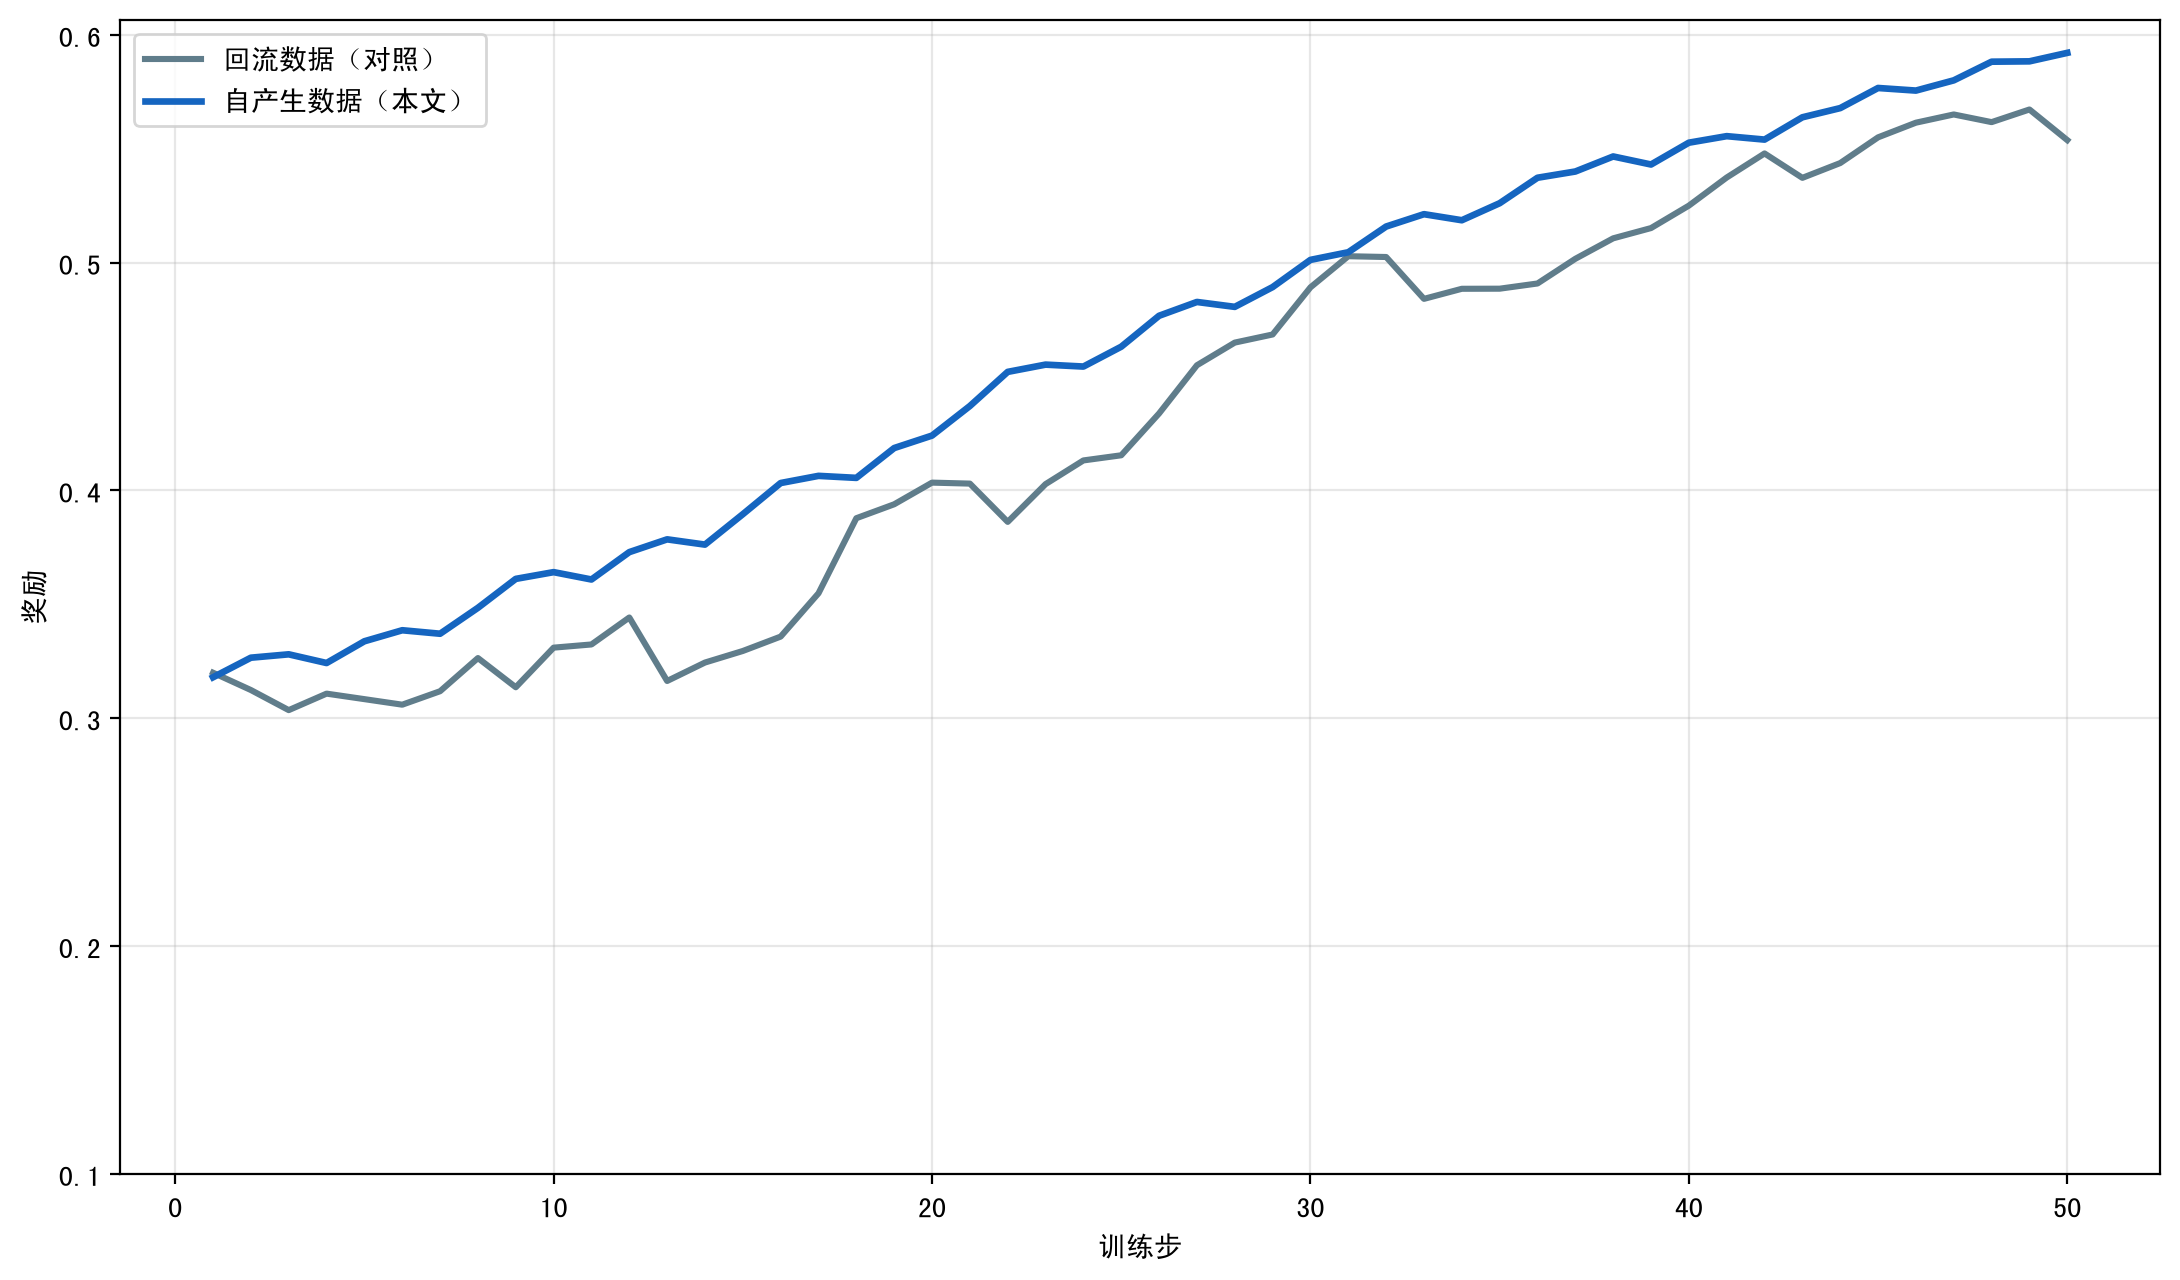
\includegraphics[width=\columnwidth]{reward.png}
\caption{奖励均值随训练步变化（EMA 平滑）：自产生数据（本文）与回流基线对比。}
\label{fig:reward}
\end{figure}

作为伴随信号，自产生数据的组内奖励标准差随步缓慢收窄（轻微方差坍缩、Echo-Trap~\cite{echo_trap} 前兆），而基线保持平稳——自产生数据在轮次间逐渐趋同，回流数据则由外部持续注入多样性。

\subsection{能力评测}

过程指标无法单独证明能力真的提升：由于奖励口径本身随自进化演化，奖励升高可能只是系统把自己的评分刷高。为此，本文以独立于训练回路的离线评测（ClawEval 文本任务）为尺子，对比三个模型：未训练基座、回流数据训练模型、本文自进化训练模型。如图~\ref{fig:eval}，本文模型得分 0.401，明显高于未训练基座（0.370）；因评测独立于训练奖励，该提升反映的是真实的能力增益而非训练指标的虚高。生成多样性小幅下降（0.285 对基座 0.294），与训练中观测的方差坍缩一致——过程与终点指标彼此吻合。

\begin{figure}[t]
\centering
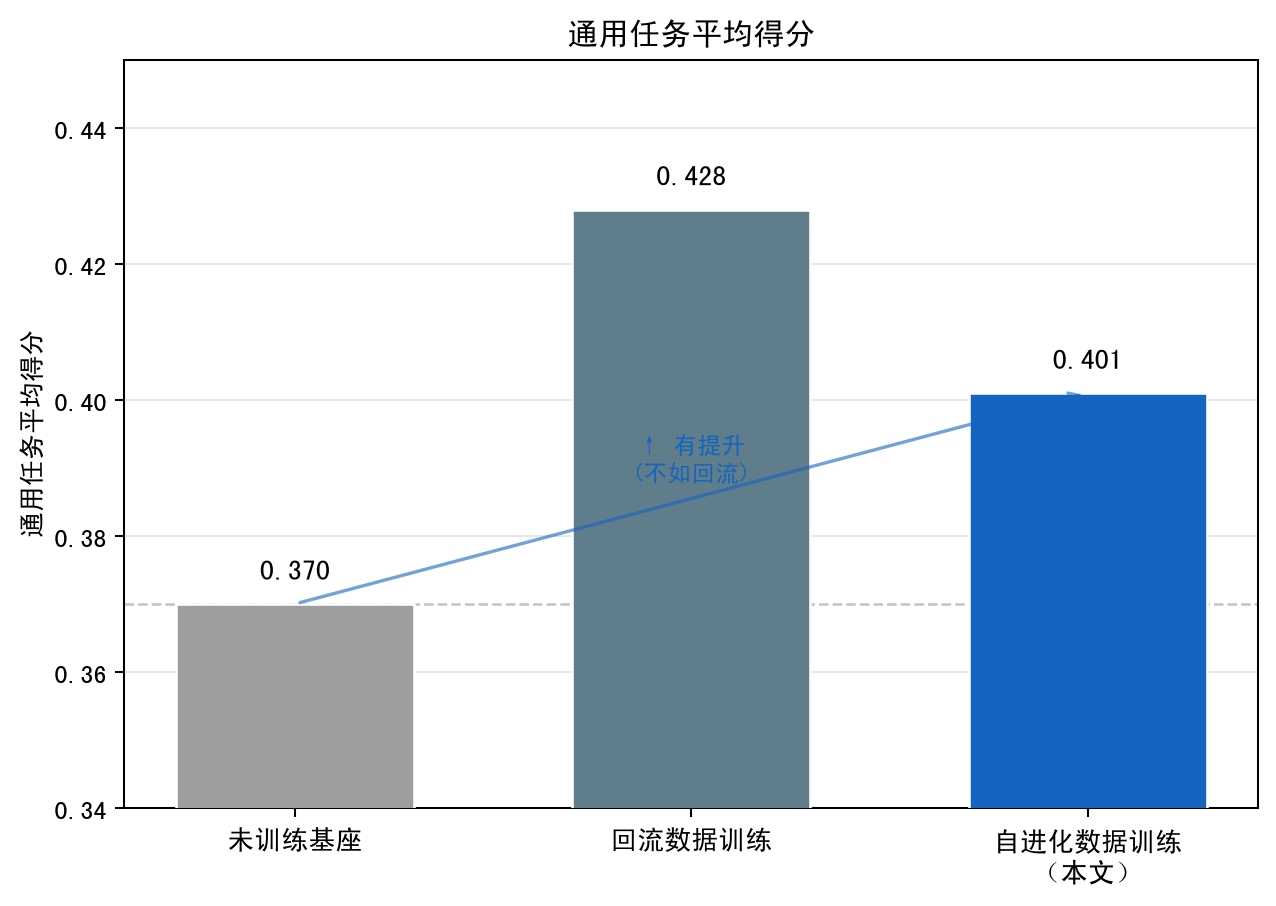
\includegraphics[width=0.85\columnwidth]{eval_score.png}
\caption{三个模型在通用任务上的平均得分；离线评测独立于训练奖励口径。}
\label{fig:eval}
\end{figure}

\section{结论}

本文提出的自进化强化学习系统同时贯通模型层面与智能体层面，将自进化的对象从“策略”单维扩展到“任务、策略、评估器、基建”四维：系统自主产生数据、将奖励锚定在确定性环境状态差分、按梯度质量筛选轨迹、并以失败案例演化评估器与基建。在 Qwen3.5-9B 上端到端运行，少量种子即可驱动完整强化学习训练、除初始种子外不依赖外部数据，独立评测确认了相对未训练基座的真实能力提升。多模态扩展、多样性正则与更大规模的训练是自然的后续方向。

\begin{thebibliography}{00}
\bibitem{self_evolution_survey} Z. Tao 等，“A survey on self-evolution of large language models,” arXiv:2404.14387, 2024.
\bibitem{self_improve} J. Huang 等，“Large language models can self-improve,” arXiv:2210.11610, 2022.
\bibitem{self_play} Z. Chen 等，“Self-play fine-tuning converts weak language models to strong language models,” arXiv:2401.01335, 2024.
\bibitem{self_rewarding} W. Yuan 等，“Self-rewarding language models,” arXiv:2401.10020, 2024.
\bibitem{rlaif} H. Lee 等，“RLAIF: Scaling RLHF with AI feedback,” arXiv:2309.00267, 2023.
\bibitem{absolute_zero} A. Zhao 等，“Absolute Zero: Reinforced self-play reasoning with zero data,” arXiv:2505.03335, 2025.
\bibitem{reward_hacking_def} J. Skalse 等，“Defining and characterizing reward hacking,” in NeurIPS, 2022.
\bibitem{reward_overoptimization} L. Gao, J. Schulman, J. Hilton, “Scaling laws for reward model overoptimization,” arXiv:2210.10760, 2022.
\bibitem{grpo} Z. Shao 等，“DeepSeekMath,” arXiv:2402.03300, 2024.
\bibitem{react} S. Yao 等，“ReAct: Synergizing reasoning and acting in language models,” arXiv:2210.03629, 2022.
\bibitem{codeact} X. Wang 等，“Executable code actions elicit better LLM agents,” arXiv:2402.01030, 2024.
\bibitem{dapo} Q. Yu 等，“DAPO: An open-source LLM reinforcement learning system at scale,” arXiv:2503.14476, 2025.
\bibitem{echo_trap} Z. Wang 等，“RAGEN: Understanding self-evolution in LLM agents via multi-turn RL,” arXiv:2504.20073, 2025.
\bibitem{camel} G. Li 等，“CAMEL: Communicative agents for `mind' exploration of large language model society,” arXiv:2303.17760, 2023.
\bibitem{llm_judge} L. Zheng 等，“Judging LLM-as-a-judge with MT-Bench and Chatbot Arena,” arXiv:2306.05685, 2023.
\bibitem{r_zero} C. Huang 等，“R-Zero: Self-evolving reasoning LLM from zero data,” arXiv:2508.05004, 2025.
\bibitem{voyager} G. Wang 等，“Voyager: An open-ended embodied agent with large language models,” arXiv:2305.16291, 2023.
\bibitem{reflexion} N. Shinn 等，“Reflexion: Language agents with verbal reinforcement learning,” arXiv:2303.11366, 2023.
\end{thebibliography}

\end{document}
